
\chapter{Diseño del Framework}
\label{cap:descripcionTrabajo}

El objetivo principal de este Trabajo de Fin de Grado es facilitar el diseño de enemigos en videojuegos de plataformas en 2D, permitiendo que diseñadores sin conocimientos de programación puedan crear comportamientos complejos de manera visual e intuitiva. Para ello, se ha desarrollado una herramienta sobre el motor \textit{Unity} que implementa un framework modular basado en componentes de comportamiento reutilizables.\\

Este capítulo describe el diseño conceptual de ese framework. En primer lugar, se analiza el contexto en el que se enmarca la herramienta y su utilidad dentro del desarrollo de videojuegos. Para ello, se presentan varios títulos de referencia y se identifican patrones comunes en el diseño de enemigos. A continuación, se explica cómo se estructura el framework, qué elementos lo componen y qué principios han guiado su desarrollo. Finalmente, se muestran ejemplos de aplicación que ilustran su uso en distintos tipos de enemigos.\\

Como se señala en \citet{Build_a_Bad_Guy_Workshop}, los enemigos bien diseñados son clave para evitar que los niveles queden planos y, en consecuencia, aburridos para el jugador. Un buen diseño de enemigos va más allá de poner un obstáculo en el camino: aporta dinamismo, construye la atmósfera del juego e incluso contribuye a la narrativa. Un enemigo puede requerir estrategias específicas para vencerlo o tener comportamientos complejos que enriquecen la experiencia del jugador.\\

El framework propuesto busca facilitar la creación de este tipo de enemigos inteligentes en 2D mediante una colección de comportamientos básicos y combinables. Está orientado a diseñadores, estudiantes o desarrolladores que deseen construir enemigos sin necesidad de escribir código, fomentando así una separación clara entre los roles de diseño y programación.\\


\section{Análisis de enemigos en videojuegos}
El análisis de diversos documentos muestra que la mejor forma de hacer que un enemigo destaque y aporte valor al juego es dotarlo de comportamientos únicos. Cada enemigo se define por una combinación específica de estos comportamientos, que determinan lo que puede o no puede hacer, y permiten diferenciarlo de otros. A lo largo del tiempo, estos comportamientos se han vuelto más sofisticados, lo que ha aumentado también la complejidad del trabajo de diseño. Para abordar esta dificultad, se ha propuesto una herramienta basada en comportamientos sencillos y precisos, que reduce la carga de trabajo sin sacrificar expresividad.\\

En este contexto, se entiende por enemigo cualquier entidad que represente una amenaza o dificultad para el jugador, afectando negativamente su progreso dentro del juego. Esto incluye no solo enemigos clásicos como soldados o monstruos, sino también elementos del entorno como pinchos, lava u obstáculos móviles. Asimismo, se ha optado por segmentar los enemigos según sus comportamientos, tratando como entidades separadas aquellos elementos que tradicionalmente se considerarían un único enemigo por su presentación conjunta. Por ejemplo, una tubería y una gota de ácido, o un pistolero y sus balas, se modelan de forma independiente en nuestro framework, ya que sus lógicas de comportamiento son autónomas y distintas.\\

Para fundamentar el diseño de esta herramienta, se ha realizado un análisis de los enemigos distintos videojuegos de plataformas en 2D. Los títulos seleccionados fueron \textit{Hollow Knight}, \textit{Blasphemous} y \textit{Bzzzt}. En los dos primeros se examinó el comportamiento individual de enemigos comunes (excluyendo jefes), mientras que el tercero se utilizó como caso de validación para comprobar que los comportamientos identificados eran suficientes para modelar los enemigos más frecuentes del juego.\\

Estos enemigos han sido seleccionados por su simplicidad estructural y su potencial para ser descompuestos en comportamientos básicos reutilizables dentro del framework.
\subsection{Hollow Knight}
\textit{Hollow Knight} es un \emph{Metroidvania} en 2D desarrollado y auto publicado por el estudio australiano \emph{Team Cherry}\footnote{\url{https://www.teamcherry.com.au/}}. Su versión inicial para ordenador se lanzó en 2017. El jugador controla al \textit{Caballero}, que explora un reino subterráneo de insectos abandonado. Derrotando enemigos por medio de distintas habilidades que se van desbloqueando, se descubre el mundo y los secretos que este oculta.\\

A continuación se describen algunos de los enemigos estudiados:
\begin{itemize}
	\item \textbf{Reptacillo:} Enemigo básico que patrulla una zona caminando en línea recta y cambiando de dirección al colisionar con un obstáculo.
	\item \textbf{Cáscara errante:} Merodea pacíficamente hasta que detecta al jugador. Una vez detectado, realiza una embestida rápida en línea recta. 
	\item \textbf{Vengamosca:} Enemigo volador que permanece revoloteando en una zona determinada y que, en caso de detectar al jugador si este se acerca lo suficiente, lo perseguirá.
	\item \textbf{Gruzzer:} Enemigo volador que cambia de dirección únicamaente al golpearse con paredes y objetos.
\end{itemize}

\subsection{Blasphemous}
Desarrollado por el estudio sevillano \emph{The Game Kitchen}\footnote{\url{https://thegamekitchen.com/}} y publicado por Team17, \textit{Blasphemous}\footnote{\url{https://thegamekitchen.com/blasphemous/}} llegó a Windows, Nintendo Switch, PlayStation 4 y Xbox One el 10 de septiembre de 2019. El jugador encarna al \textit{Penitente} el único superviviente en la tierra de Cvstodi. Atrapado en un ciclo de penitencia de muerte y resurrección, el Penitente tendrá que liberar al mundo del destino que le espera.\\

Como enemigos analizados en este caso encontramos:
\begin{itemize}
	\item \textbf{Enraged Pilgrim:} Enemigo terrestre que permanece inmóvil hasta que el jugador entra en un rango de detección determinado. Una vez activado, comienza a caminar lentamente hacia el jugador. Cuando se encuentra a corta distancia, ejecuta un ataque cuerpo a cuerpo utilizando un cuchillo.
	\item \textbf{Spikes:} Elemento estático del entorno que actúa como obstáculo letal. Consiste en una superficie con pinchos que, al entrar en contacto con el jugador, provoca su derrota inmediata. 
	\item \textbf{Shooting Trap:} Trampa fija que lanza proyectiles a través de una abertura frontal. Dispara de forma continua en una única dirección, con una frecuencia constante y sin necesidad de detección del jugador.
	\item \textbf{Acolyte:} Enemigo terrestre que patrulla una zona y, al detectar al jugador, se detiene brevemente para luego realizar una embestida en su dirección.
\end{itemize}


\subsection{Bzzzt}

\textit{Bzzzt}\footnote{\url{https://store.steampowered.com/app/1293170/BZZZT/}} es un plataformas de acción de estética retro desarrollado casi íntegramente por el checo Karel Matějka  y publicado por Cinemax. Se estrenó para PC en noviembre de 2023 y para Nintendo Switch en septiembre de 2024. el jugador, en el papel de un robot, debe frustrar los planes del villano Badbert y rescatar a sus creadores, los doctores Emily y Norbert, atravesando 52 niveles llenos de trampas y enemigos de estilo arcade.

En este caso los enemigos son:
\begin{itemize}
	\item \textbf{Saw Drone:} Enemigo volador que se desplaza siguiendo un patrón circular o semicircular. Causa daño al contacto y no reacciona a la presencia del jugador.
	\item \textbf{Cannon Turret:} Trampa fija que dispara proyectiles a intervalos regulares en una dirección determinada. No detecta al jugador, pero su ritmo constante obliga al jugador a calcular el momento adecuado para pasar.
	\item \textbf{Walking Bot:} Enemigo terrestre que patrulla horizontalmente entre dos límites. Cambia de dirección al chocar con obstáculos o al llegar al borde de la plataforma.
	\item \textbf{Chasing Bot:} Enemigo que, al detectar al jugador en un cierto rango, cambia su patrón de patrulla por una persecución directa. Su velocidad puede aumentar durante la persecución.
	\item \textbf{Spike Block:} Obstáculo estático que actúa como una trampa pasiva. Causa daño letal al jugador si entra en contacto con él. Puede estar en el suelo, techo o paredes.
\end{itemize}

\subsection{Comportamientos relevantes detectados}

El análisis de los enemigos presentes en los tres videojuegos permitió identificar una serie de patrones de comportamiento comunes entre ellos:

\begin{itemize}
	\item \emph{Patrulla:} Movimiento horizontal constante entre dos puntos, cambiando de dirección al chocar con un obstáculo o al alcanzar un borde. Este comportamiento está presente en enemigos como el Reptacillo (\textit{Hollow Knight}), el Acolyte (\textit{Blasphemous}) y el Walking Bot (\textit{Bzzzt}).
	\item \emph{Embestida lineal:} Una vez que detectan al jugador, interrumpen su comportamiento actual y se lanzan rápidamente en línea recta para atacarlo. Se observa en enemigos como la Cáscara errante (\textit{Hollow Knight}) y el Acolyte (\textit{Blasphemous}).
	\item \emph{Persecución:} Enemigos que, al detectar al jugador, comienzan a seguirlo directamente, adaptando su trayectoria en tiempo real. Este comportamiento se encuentra en la Vengamosca (\textit{Hollow Knight}) y el Chasing Bot (\textit{Bzzzt}).
	\item \emph{Torreta:} Disparo continuo o periódico de proyectiles en una dirección fija, sin depender de la posición del jugador. Representado por la Shooting Trap (\textit{Blasphemous}) y la Cannon Turret (\textit{Bzzzt}).
	\item \emph{Rotación fija:} Movimiento circular o semicircular alrededor de un punto o eje, sin modificar el patrón según la presencia del jugador. Ejemplificado por el Saw Drone (\textit{Bzzzt}).
	\item \emph{Trampa estática letal:} Elementos del entorno que causan la derrota del jugador al contacto directo, sin movimiento ni detección. Este patrón se encuentra en los Spikes (\textit{Blasphemous}) y el Spike Block (\textit{Bzzzt}).
\end{itemize}

\section{Conclusiones del análisis y definición del framework}

El estudio de los enemigos presentes en los videojuegos \textit{Hollow Knight}, \textit{Blasphemous} y \textit{Bzzzt} permitió identificar una serie de patrones recurrentes en su comportamiento. Estos patrones han sido agrupados en categorías comunes, lo que permite abstraer el comportamiento de cada enemigo en términos funcionales.\\

A partir de esta observación, se ha definido un framework modular que permite construir enemigos a partir de tres componentes fundamentales:

\begin{itemize}
  \item \textbf{Sensores:} Son los mecanismos que permiten a un enemigo percibir información de su entorno. Definen condiciones de activación para ciertos comportamientos.
  \item \textbf{Actuadores:} Son las acciones que un enemigo puede ejecutar en un momento determinado. Incluyen movimientos, ataques y generación de nuevos enemigos, entre otros.
  \item \textbf{Sistema de daño:} Determina cómo un enemigo recibe y procesa el daño, incluyendo la interacción con elementos ofensivos del entorno (como ataques del jugador), invulnerabilidad temporal, reacciones visuales o físicas, y la gestión de su salud.
\end{itemize}

Esta separación en sensores, actuadores y daño permite una construcción flexible y reutilizable de comportamientos. En lugar de diseñar enemigos de forma específica para cada situación, es posible combinar estos elementos de forma modular para crear una gran variedad de comportamientos complejos.\\

En esta sección, se presentan los principales \textbf{actuadores} identificados a partir del análisis anterior, que constituyen la base para definir el comportamiento activo de los enemigos. Posteriormente, se describirán los \textbf{sensores}, encargados de activar estos actuadores según las condiciones del entorno. A continuación, se detalla el sistema de \textbf{daño}, necesario para gestionar las interacciones ofensivas entre el jugador y los enemigos y sus consecuencias.\\

Por último, una vez definidos los sensores, actuadores y el sistema de daño como elementos fundamentales del comportamiento enemigo, se introduce el concepto de \textbf{estado}, entendido como una combinación coherente de acciones que un enemigo puede ejecutar en un momento determinado, encapsuladas en los actuadores. Esta noción permite estructurar y organizar el comportamiento de forma modular. A partir de ello, se construye la Máquina de Estados Finita (FSM), el componente central de la lógica de control del enemigo. Cada enemigo contará con su propia FSM, la cual gestiona sus diferentes estados y las transiciones entre ellos en función de las señales recibidas por los sensores. Esta arquitectura permite representar comportamientos complejos de manera flexible, escalable y reutilizable dentro del framework propuesto.\\

\section{Actuadores}
\label{subsec:acciones}
Hace referencia a un conjunto de movimientos y habilidades que definen lo que un enemigo puede hacer en el videojuego. Esto incluye distintos tipos de desplazamientos y la capacidad de crear otros enemigos de forma independiente (spawners). Estas habilidades no siempre son 
compatibles entre sí, por lo que es necesario especificar las relaciones de compatibilidad mediante una tabla.\\

En nuestro diseño, distinguimos dos tipos principales de actuadores: de movimiento, que definen cómo se desplazan los enemigos por el entorno, y los spawners, que les permiten generar otras entidades dentro del juego.

\subsection{Movimiento}
Podemos definir el término movimiento como el desplazamiento o cambio de posición de un enemigo dentro del juego. Sin embargo, el concepto de movimiento también puede aplicarse en el caso de enemigos que permanecen en una posición fija, haciendo referencia a la ausencia de éste. Los movimientos son fundamentales para definir el comportamiento de los personajes, ya que permiten la interacción con el jugador y el entorno.\\

A continuación se muestran todos los movimientos diseñados, junto con una breve descripción.
\begin{itemize}
  \item \textbf{Horizontal}: Desplaza al enemigo horizontalmente, hacia la izquierda o derecha.
    \item \textbf{Vertical}: Desplaza al enemigo verticalmente, hacia arriba o abajo.
    \item \textbf{Directional}: Mueve al enemigo en una dirección definida por un ángulo, siendo el valor cero un movimiento hacia la derecha e incremental en el sentido antihorario.
    \item \textbf{Circular}: Hace que el enemigo siga un movimiento circular alrededor de un punto, describiendo una circunferencia cerrada si el ángulo es igual a 360 y, en caso de ser menor, actuando como péndulo.
    \item \textbf{Move To A Point}\label{sec:MoveToAPoint}: Dirige al enemigo hacia puntos concretos no actualizables. Se puede configurar por medio de una lista, donde se indican los puntos concretos a recorrer o por medio de un área, donde se eligirá aleatoriamente un punto y al llegar a él, se escogerá otro.
    \item \textbf{Move To An Object}: Desplaza al enemigo hacia una entidad que puede estar en movimiento.
    \item \textbf{Spline Follower} \label{act:splinefollower}: Permite al enemigo seguir una trayectoria definida por una curva suave que se genera a partir de un conjunto de puntos de control, denominada \textit{spline}. Una spline es una curva que conecta estos puntos de control mediante segmentos continuos y suavizados. Cada punto puede incluir manejadores (handlers) para controlar la tangente de entrada y salida, lo que permite ajustar con precisión la forma de la curva. Esta técnica proporciona trayectorias fluidas y naturales, ideales para movimientos complejos o decorativos.

\end{itemize}

Todos los tipos de movimiento pueden configurarse para ejecutarse de forma acelerada. Para ello, se emplea una función de aceleración/suavizado (\textit{Easing Function}), una función que define cómo varían en un tiempo definido tanto la velocidad como la posición del enemigo. \\
Dependiendo del tipo de movimiento, esta función puede aplicarse de dos formas:\\

\begin{itemize}
\item En movimientos como \textbf{Horizontal}, \textbf{Vertical}, \textbf{Directional} o \textbf{Circular} (Figura \ref{fig:EasingFuntionVel}), la \textit{Easing Function} afecta principalmente a la velocidad, modificándola teniendo en cuenta una velocidad objetivo y un tiempo para llegar a ella.
\item En movimientos como \textbf{Move To A Point} y \textbf{Move To An Object} (Figura \ref{fig:EasingFunction}), la \textit{Easing Function} influye directamente en la interpolación de la posición, alterando cómo el enemigo se desplaza entre el origen y el destino en un tiempo determinado.
\end{itemize}

Este enfoque permite controlar el dinamismo del movimiento, proporcionando una mayor expresividad y naturalidad en el comportamiento de los enemigos. Por ello, se incluye un catálogo\footnote{\url{https://gist.github.com/cjddmut/d789b9eb78216998e95c}} de distintas \textit{Easing Functions} que permite variar la forma en que se definen y perciben los movimientos.\\

La influencia de las \textit{Easing Functions} en cada tipo de movimiento, así como las imágenes utilizadas para ilustrarlas, se explicará con mayor profundidad en el apartado de Implementación (Capítulo~\ref{cap:implementacion}).

\begin{figure}[t]
	\centering
	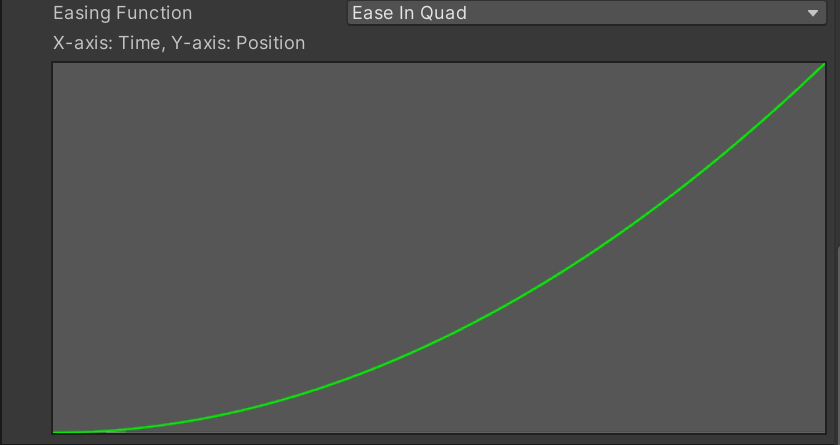
\includegraphics[height=7cm]{Imagenes/EasingFunction.png}
	\caption{Easing Function que describe la variación de la posición de un objeto con el movimiento Move To An Object}
	\label{fig:EasingFunction}
\end{figure}

\begin{figure}[t]
	\centering
	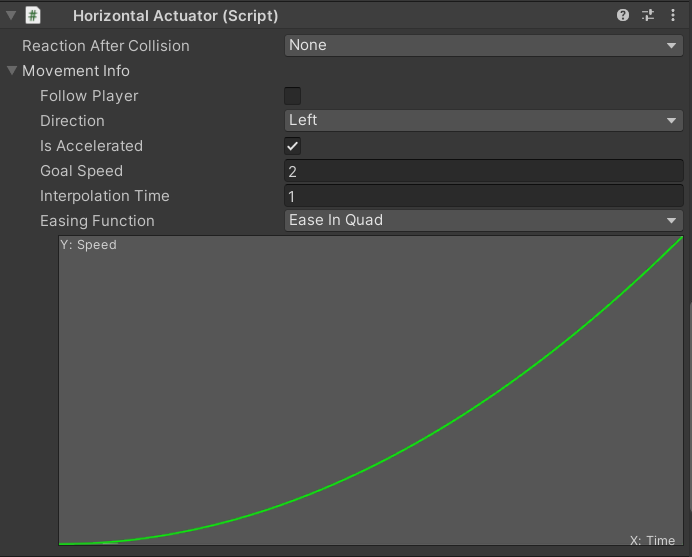
\includegraphics[height=7cm]{Imagenes/HorizontalMovementAccelerated.png}
	\caption{Easing Function que describe la variación de la velocidad de un objeto con el movimiento Horizontal}
	\label{fig:EasingFuntionVel}
\end{figure}

\subsection{Spawner}
\label{subsec:spawner}

\textit{Spawnear} es la capacidad que poseen algunos enemigos para generar otras unidades enemigas de forma independiente, actuando como entidades que crean nuevas amenazas dentro del juego. Esta funcionalidad añade dinamismo y complejidad a la jugabilidad, permitiendo, por ejemplo, que una torreta dispare proyectiles o que un enemigo invoque aliados en mitad del combate.

Para diseñar un sistema de generación versátil, es necesario establecer un conjunto de reglas claras que definan cómo y cuándo debe producirse esta generación. A continuación, se plantean estas reglas como preguntas clave de diseño:

\begin{itemize}
    \item \textbf{¿Con qué frecuencia se generan nuevas unidades?} \\
    Cada entidad generadora establece un intervalo de espera entre una generación y la siguiente. Este intervalo define el ritmo con el que aparecen las nuevas unidades, afectando directamente al nivel de presión sobre el jugador.

    \item \textbf{¿Cuántas unidades se pueden generar?} \\
    El sistema permite limitar la cantidad total de unidades generadas o, si se desea, habilitar una generación ilimitada. Esta decisión influye tanto en el balance como en la duración del desafío que representa el generador.

    \item \textbf{¿Dónde aparecen las unidades generadas?} \\
    Cada entidad generadora puede estar asociada a uno o varios puntos del escenario. En cada ciclo de generación, una nueva unidad aparece en estos puntos previamente definidos, lo que permite controlar espacialmente el comportamiento del sistema.

    \item \textbf{¿Cómo se produce la generación de forma visual o interactiva?} \\
    El sistema de generación puede integrarse con las animaciones de la entidad generadora. Esto permite sincronizar la aparición de nuevas unidades con acciones visuales específicas (como una animación de ataque), aportando coherencia visual y reforzando la inmersión del jugador.
\end{itemize}

El comportamiento del generador se rige por estas reglas, evaluando de forma continua si las condiciones necesarias se cumplen. Solo entonces se permite la creación de nuevas unidades, asegurando que el sistema se mantenga bajo control y alineado con la experiencia de juego deseada.

\subsection{Compatibilidad}
La versatilidad de la herramienta se potencia al permitir la combinación de diversos actuadores simultáneamente. En este sentido, un enemigo podría perfectamente desplazarse horizontalmente mientras activa un spawner para generar secuaces. Esta sinergia entre actuadores (movimientos y spawners) enriquece la complejidad del comportamiento y abre un abanico de posibilidades creativas para los diseñadores.\\

No obstante, es crucial reconocer que no todas las combinaciones de acciones resultan coherentes o deseables desde la perspectiva del diseño del juego. Por ejemplo, intentar realizar un movimiento vertical mientras se está definido un movimiento circular podría generar comportamientos visuales o de jugabilidad no intencionados. \\

Para clarificar estas interdependencias y asegurar la coherencia en la configuración de los enemigos, se ha elaborado la \textit{Tabla~\ref{tab:compatibilidad}} de compatibilidad. Esta tabla actuará como una guía visual e intuitiva, indicando qué combinaciones de movimientos y la activación de spawners son factibles y recomendadas, permitiendo a los diseñadores construir enemigos con comportamientos complejos pero lógicos y bien definidos.

\begin{table}[!h]
    \centering
    \caption{Matriz de compatibilidad de movimientos}
    \label{tab:compatibilidad}
    \resizebox{\textwidth}{!}{%
    \begin{tabular}{|l|c|c|c|c|c|c|c|c|}
    \hline
    \textbf{} & \textbf{Horizontal} & \textbf{Vertical} & \textbf{Directional} & \textbf{Circular} & \textbf{Move To A Point} & \textbf{Move To An Object} & \textbf{Spline Follower} & \textbf{Spawner} \\
    \hline
    \textbf{Horizontal} & \cellcolor{gray!40} & \cellcolor{gray!40} & \cellcolor{gray!40} & \cellcolor{gray!40} & \cellcolor{gray!40} & \cellcolor{gray!40} & \cellcolor{gray!40} & \cellcolor{gray!40} \\
    \hline
    \textbf{Vertical} & \cellcolor{green!70} & \cellcolor{gray!40} & \cellcolor{gray!40} & \cellcolor{gray!40} & \cellcolor{gray!40} & \cellcolor{gray!40} & \cellcolor{gray!40} & \cellcolor{gray!40} \\
    \hline
    \textbf{Directional} & \cellcolor{red!70} & \cellcolor{red!70} & \cellcolor{gray!40} & \cellcolor{gray!40} & \cellcolor{gray!40} & \cellcolor{gray!40} & \cellcolor{gray!40} & \cellcolor{gray!40} \\
    \hline
    \textbf{Circular} & \cellcolor{red!70} & \cellcolor{red!70} & \cellcolor{red!70} & \cellcolor{gray!40} & \cellcolor{gray!40} & \cellcolor{gray!40} & \cellcolor{gray!40} & \cellcolor{gray!40} \\
    \hline
    \textbf{Move To A Point} & \cellcolor{red!70} & \cellcolor{red!70} & \cellcolor{red!70} & \cellcolor{red!70} & \cellcolor{gray!40} & \cellcolor{gray!40} & \cellcolor{gray!40} & \cellcolor{gray!40} \\
    \hline
    \textbf{Move To An Object} & \cellcolor{red!70} & \cellcolor{red!70} & \cellcolor{red!70} & \cellcolor{red!70} & \cellcolor{red!70} & \cellcolor{gray!40} & \cellcolor{gray!40} & \cellcolor{gray!40} \\
    \hline
    \textbf{Spline Follower} & \cellcolor{red!70} & \cellcolor{red!70} & \cellcolor{red!70} & \cellcolor{red!70} & \cellcolor{red!70} & \cellcolor{red!70} & \cellcolor{gray!40} & \cellcolor{gray!40} \\
    \hline
    \textbf{Spawner} & \cellcolor{green!70} & \cellcolor{green!70} & \cellcolor{green!70} & \cellcolor{green!70} & \cellcolor{green!70} & \cellcolor{green!70} & \cellcolor{green!70} & \cellcolor{gray!40} \\
    \hline
    \end{tabular}
    }
    \vspace{0.5em}
    \caption*{\textbf{Leyenda de colores:} \textcolor{green!70!black}{Verde} = combinación compatible; \textcolor{red!70!black}{Rojo} = combinación no compatible; \textcolor{gray!70!black}{Gris} = combinación redundante.}
\end{table}

\section{Sensores}
\label{subsec:sensores}
El término sensor se define como los mecanismos mediante los cuales los personajes interactúan con su entorno y entre sí.
Podemos definir el término sensor como el elemento que sirve para que el enemigo conozca el entorno y reciba información de los cambios que se producen en el mismo. Son los responsables de activar las transiciones entre estados, es decir, se encargan de cambiar de un comportamiento predefinido a otro.
A continuación se enumerarán los diferentes sensores disponibles en la herramienta.
\begin{itemize}
	\item \textbf{Area}: Detecta si un objeto entra o sale en una zona de detección.
	\item \textbf{Collision}: Detecta colisiones físicas con otros objetos.
	\item \textbf{Distance}: Evalúa si un objeto se encuentra dentro o fuera de una distancia específica con respecto a otro. Esta condición puede interpretarse de dos maneras distintas según su configuración:
	\begin{itemize}
	    \item \textit{Distancia absoluta}: Se mide la distancia total, sin importar la dirección. Es útil para detectar proximidad general.
	    \item \textit{Distancia por eje}: Permite verificar la distancia solo en un eje determinado (por ejemplo, solo en el eje X), ignorando la separación en el Y. Esta modalidad resulta útil para detectar alineamientos específicos (como estar “a la misma altura” o “en la misma línea horizontal”).
	\end{itemize}
	\item \textbf{Time}: Detecta cuando ha transcurrido un tiempo determinado.
\end{itemize}
\section{Daño}
\label{subsec:dano}
Se define daño como la consecuencia negativa que recibe una entidad con respecto a su vida. Esto se produce como la consecuencia de una colisión entre dos entidades del juego, una que hace daño y otra que lo recibe.\\
Existen diferentes tipos de daño y parámetros específicos que determinan cómo las entidades reciben, emiten y procesan daño.
La primera consideración que hay que tener en cuenta es que el daño no es bidireccional, lo que implica que un volumen que recibe daño no tiene por qué emitir daño. Para reflejar esta diferenciación se han creado los siguientes dos componentes:
\begin{itemize}
    \item \textbf{Damage Sensor}: Detecta si el objeto ha recibido daño.
    \item \textbf{Damage Emitter}: Efectúa daño.
\end{itemize}

Además, se puede distinguir entre tres tipos de daños:
\begin{itemize}
    \item \textbf{Instantáneo:} Aplica una única vez el daño al tener contacto.
    \item \textbf{De Permanencia:} Inflige daño continuo mientras haya contacto, definiendo la cantidad y la frecuencia de aplicación de daño.
    \item \textbf{Residual:} Aplica daño inicial y luego daño periódico tras el contacto, definiendo cantidades, frecuencia de aplicación y número de aplicaciones.
\end{itemize}

\section{Máquina de Estados Finita}
\label{sec:fsm}

La Máquina de Estados Finita (FSM, por sus siglas en inglés \textit{Finite State Machine}) constituye el núcleo de la lógica de comportamiento de los enemigos en el framework propuesto. Su función principal es organizar y controlar el flujo de acciones que puede realizar un enemigo a lo largo del tiempo, de forma estructurada, flexible y escalable. Cada enemigo cuenta con su propia instancia de FSM.\\

La FSM se compone de un estado inicial, el cual encapsula una configuración concreta de comportamiento, así como sus posibles \textbf{transiciones} hacia otros estados. Esta estructura permite modelar de forma clara y modular la lógica interna de cada enemigo.

\subsection{Estado}
\label{subsec:estado}

Un estado representa una situación concreta en la que se encuentra el enemigo, definida por un conjunto específico de actuadores que se ejecutan mientras permanece en dicho estado. Además, cada estado incluye sus propias transiciones y puede incorporar emisores de daño.\\

En particular, cada estado puede incluir uno o varios emisores de daño, que son los encargados de infligir daño a otras entidades del juego durante la ejecución del estado. Esto permite, por ejemplo, que un enemigo cause daño únicamente cuando se encuentra atacando, o que un área peligrosa esté activa solo durante determinados comportamientos.

\subsubsection{Transiciones}

Cada estado contiene sus propias transiciones, que determinan a qué otros estados puede cambiar el enemigo y bajo qué condiciones. Estas condiciones están definidas por los sensores, que detectan información relevante del entorno.\\

Cuando se cumple la condición de una transición, el estado actual cede el control al nuevo estado indicado, permitiendo una evolución fluida y dinámica del comportamiento del enemigo.

\begin{figure}[h]
	\centering
	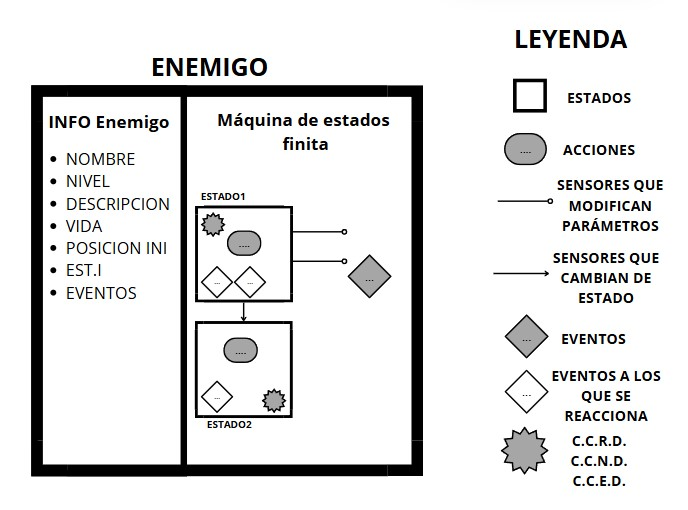
\includegraphics[height=5cm]{Imagenes/EnemigoGeneral.png}
	\caption{Ejemplo de estructura general de un enemigo basado en FSM.}
	\label{fig:EnemigoGeneral}
\end{figure}
\subsection{Sincronización con las animaciones}
\label{subsec:animaciones_fsm}

El comportamiento de un enemigo no solo debe ser funcional, sino también comprensible y coherente para el jugador. Por ello, los actuadores incluidos en cada estado pueden modificar la representación visual del enemigo mediante animaciones. Esta sincronización garantiza que lo que el enemigo está haciendo internamente, también se refleje externamente de forma clara.\\

Cada vez que un enemigo realiza una acción específica de un actuador —por ejemplo, \textit{spawnear} una entidad, o pasar de deambular en una zona a perseguir al jugador— su animación cambia para representar visualmente esa transición. Así, el jugador puede anticipar acciones, reconocer patrones de comportamiento y reaccionar en consecuencia.\\

Además, ciertos eventos clave como recibir daño o morir, activan animaciones específicas que refuerzan su impacto y aportan una mayor riqueza expresiva al sistema. Estas animaciones no son decorativas: forman parte esencial de la comunicación entre el enemigo y el jugador.\\

Este enfoque integrador entre comportamiento y apariencia permite diseñar enemigos no solo eficaces a nivel de juego, sino también consistentes desde el punto de vista estético y narrativo.\\

Se darán detalles de como funciona esta integración en la sección~\ref{sec:animation}.

\section{Ejemplos de uso}
La división en actuadores, sensores, módulos de daño y estados permite construir enemigos complejos de forma modular, reutilizable y visualmente comprensible, sin necesidad de escribir código. A través de la combinación de estos elementos básicos, es posible definir distintos tipos de enemigos, cada uno con su propio comportamiento, nivel de amenaza e impacto sobre el jugador.\\

En esta sección se presentan ejemplos representativos de enemigos diseñados mediante la combinación de estos componentes. Estos ejemplos no son únicos, pero ilustran cómo el sistema permite definir comportamientos diversos de forma coherente y escalable.\\

Cabe destacar que estos enemigos están inspirados directamente en los patrones y casos identificados durante el análisis previo. En dicha fase se observaron distintas tipologías de enemigos en juegos de plataformas —desde amenazas constantes en movimiento, hasta enemigos estáticos con ataques periódicos o comportamientos reactivos— y aquí se muestra cómo tales comportamientos pueden reproducirse y estructurarse utilizando el sistema propuesto. El objetivo es demostrar que el marco de diseño desarrollado no solo es teóricamente sólido, sino también aplicable de forma práctica a casos reales observados en juegos comerciales.\\

Aunque algunos términos aún no han sido desarrollados, todos serán introducidos más adelante en el capítulo de implementación.

Cada enemigo combina los siguientes elementos de diseño:
\begin{itemize}
    \item Una lógica basada en una máquina de estados, que permite cambiar su comportamiento (si es necesario) en función del entorno del enemigo.
    \item Acciones específicas definidas por actuadores.
    \item Un sistema visual coherente mediante animaciones asociadas al estado del enemigo.
    \item Un sistema de daño que define cómo y cuándo el enemigo puede hacer daño o recibirlo.
\end{itemize}

\subsection{Bouncing Bunny}

El \textit{Bouncing Bunny} (Figura\ref{fig:BouncingBunny}) representa un ejemplo clásico de enemigo patrullero, inspirado directamente en enemigos como el Reptacillo (\textit{Hollow Knight}) o el Walking Bot (\textit{Bzzzt}), ambos caracterizados por un movimiento horizontal entre dos límites definidos del escenario.\\

Este enemigo recorre continuamente un tramo en línea recta, desplazándose de izquierda a derecha a velocidad constante. Al llegar a la pared invierte automáticamente su dirección, generando un patrón de patrullaje sencillo pero efectivo.\\

Su principal función dentro del diseño del nivel es la de introducir una amenaza predecible en zonas iniciales, obligando al jugador a aprender los tiempos de movimiento y a coordinar sus saltos para evitar el contacto. Esta previsibilidad lo convierte en un enemigo ideal para fases de aprendizaje, donde el jugador comienza a familiarizarse con las mecánicas básicas del juego.\\

A nivel de comportamiento, su peligro reside en el daño que inflige al contacto, aunque su resistencia es mínima, por lo que puede ser eliminado fácilmente. Esta dualidad contribuye a establecer un ritmo de juego dinámico sin suponer un obstáculo insalvable para el jugador principiante.\\

\begin{figure}[t]
	\centering
	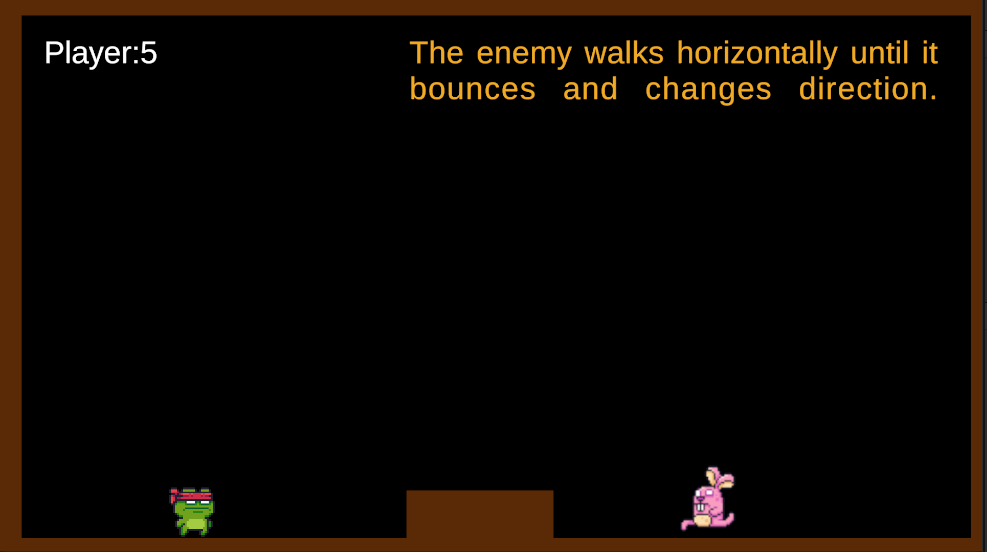
\includegraphics[height=5cm]{Imagenes/BouncingBunny.png}
	\caption{Escena de ejemplo donde observamos al enemigo en cuestión momentos antes de alcanzar la pared.}
	\label{fig:BouncingBunny}
\end{figure}

\subsection{Spinning Rocks}

El enemigo \textit{Spinning Rocks} (Figura~\ref{fig:SpinningRocks}) representa un ejemplo claro del patrón de rotación fija identificado en el análisis previo, similar al comportamiento del Saw Drone en \textit{Bzzzt}. Su función principal es la de constituir una amenaza constante basada en un movimiento predecible pero difícil de evitar, especialmente en espacios reducidos o plataformas móviles.\\

Cada unidad de este enemigo gira de forma continua alrededor de un punto central, describiendo una trayectoria circular completa. Aunque visualmente pueda interpretarse como una estructura compuesta, en realidad se trata de varias entidades independientes que orbitan de manera sincronizada, generando un entorno hostil a su alrededor.\\

La amenaza que presenta este tipo de enemigo no reside en su capacidad de persecución o ataque dirigido, sino en su mera presencia en el escenario. Al no poder ser destruido ni detenido, obliga al jugador a anticipar el patrón de movimiento y planificar cuidadosamente el momento para cruzar o interactuar con el entorno. Esta característica lo convierte en un excelente recurso para secciones de plataformas que requieren precisión y \textit{timing}.\\

A nivel de diseño, su uso está orientado a crear zonas de paso peligrosas que introducen tensión sostenida. Su predecibilidad lo hace justo, pero su invulnerabilidad lo vuelve implacable, lo que refuerza su valor como obstáculo en segmentos avanzados o de alto riesgo dentro del nivel.

\begin{figure}[t]
	\centering
	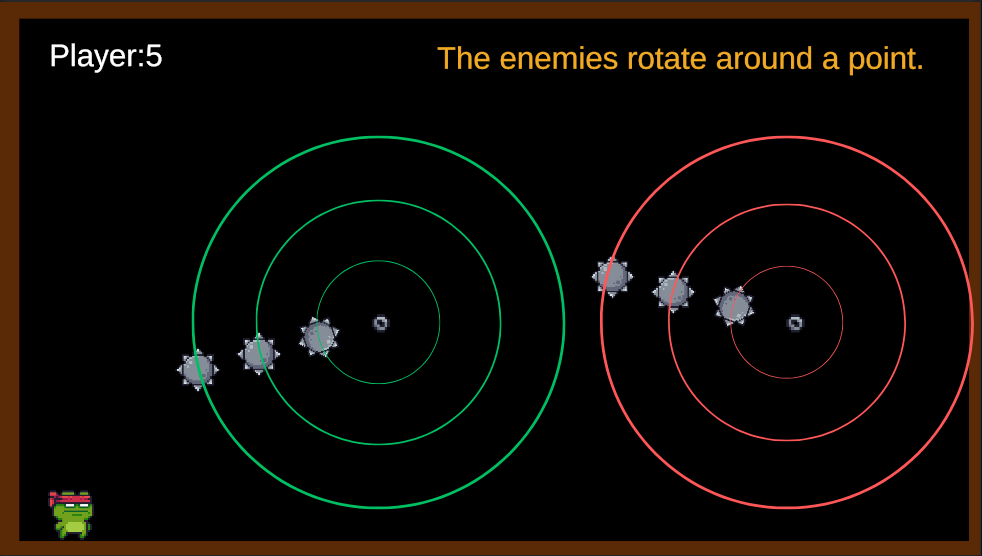
\includegraphics[height=5cm]{Imagenes/SpinningRocks.png}
	\caption{Escena de ejemplo donde se aprecian dos enemigos realizando un movimiento circular, cada uno en un sentido diferente.}
	\label{fig:SpinningRocks}
\end{figure}

\subsection{Trunk Turret}

La \textit{Trunk Turret} (Figura~\ref{fig:TrunkTurret}) es un claro ejemplo del patrón de comportamiento identificado como \emph{torreta} durante el análisis de enemigos, tal como se observa en la \textit{Shooting Trap} de \textit{Blasphemous} o la \textit{Cannon Turret} de \textit{Bzzzt}. Se trata de un enemigo completamente estático cuya principal amenaza reside en la emisión periódica de proyectiles, los cuales obligan al jugador a mantenerse en constante movimiento y adoptar un enfoque reactivo basado en la evasión.\\

A diferencia de otros enemigos móviles o interactivos, la \textit{Trunk Turret} no inflige daño directamente ni puede ser destruida. Su condición de invulnerabilidad la convierte en un elemento de peligro permanente en el escenario, generando zonas de paso peligrosas donde el jugador debe coordinar sus desplazamientos con el ritmo de disparo para evitar ser alcanzado.\\

Este tipo de enemigo funciona particularmente bien en zonas de transición o plataformas estrechas, donde el margen de error es reducido. Además, su previsibilidad rítmica aporta una capa de estrategia, ya que el jugador puede anticipar el disparo y actuar en consecuencia, generando una tensión constante sin recurrir a un comportamiento impredecible.\\

\subsubsection{Bullet}

El proyectil emitido por la \textit{Trunk Turret} se comporta como una amenaza secundaria pero letal. Se desplaza horizontalmente a velocidad constante y se destruye al colisionar con cualquier superficie o con el jugador, a quien inflige daño inmediato. Esta dinámica complementa el carácter del enemigo principal, reforzando su papel como generador de obstáculos periódicos que condicionan el movimiento del jugador.\\

La inclusión del proyectil permite ampliar la funcionalidad del enemigo sin necesidad de dotarlo de movilidad o interacción directa, lo que demuestra la versatilidad del sistema basado en componentes. Tanto la torre como la bala funcionan de forma independiente pero coordinada, lo que permite su reutilización en otros contextos o combinaciones.\\

\begin{figure}[t]
	\centering
	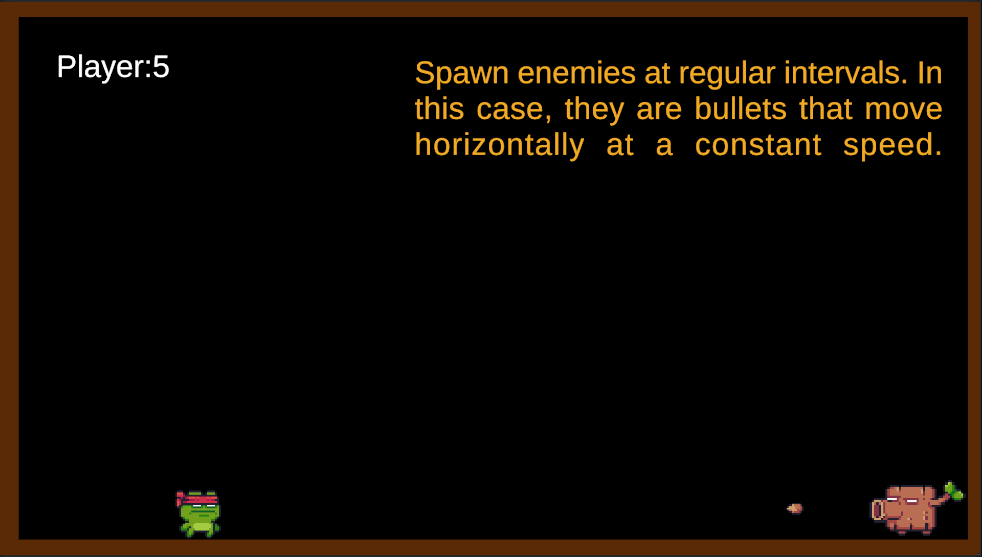
\includegraphics[height=5cm]{Imagenes/TrunkTorret.png}
	\caption{Escena de ejemplo donde se aprecia una \textit{Trunk Turret} disparando.}
	\label{fig:TrunkTurret}
\end{figure}
\subsection{Spline Chicken}

La \textit{Spline Chicken} (Figura~\ref{fig:SplineChicken}) ejemplifica una variación del patrón de patrullaje, previamente identificado. Sin embargo, a diferencia de aquellos enemigos que se desplazan en línea recta, esta gallina se mueve siguiendo una trayectoria definida, generando un movimiento continuo y cíclico alrededor de una plataforma concreta.\\

Este comportamiento introduce una dinámica distinta en el diseño del nivel. La trayectoria predefinida obliga al jugador a observar y anticipar los patrones de movimiento con mayor precisión, ya que las curvas pueden generar ángulos muertos o zonas de paso más breves. Aunque su diseño visual puede transmitir un tono humorístico, la \textit{Spline Chicken} representa una amenaza persistente: no puede ser eliminada ni detenida, y provoca daño inmediato al contacto.\\

Su presencia funciona como elemento de presión en zonas de transición o salto, donde el jugador debe sincronizar su avance con el ritmo del movimiento del enemigo. Al igual que otros enemigos invulnerables, cumple una función más cercana a la de una trampa móvil, generando tensión constante sin requerir interacción directa con el combate.\\

Este diseño demuestra cómo el marco de componentes propuesto permite extender comportamientos clásicos (como el patrullaje) a variantes más sofisticadas y visualmente interesantes, sin necesidad de redefinir estructuras complejas.\\

\begin{figure}[t]
	\centering
	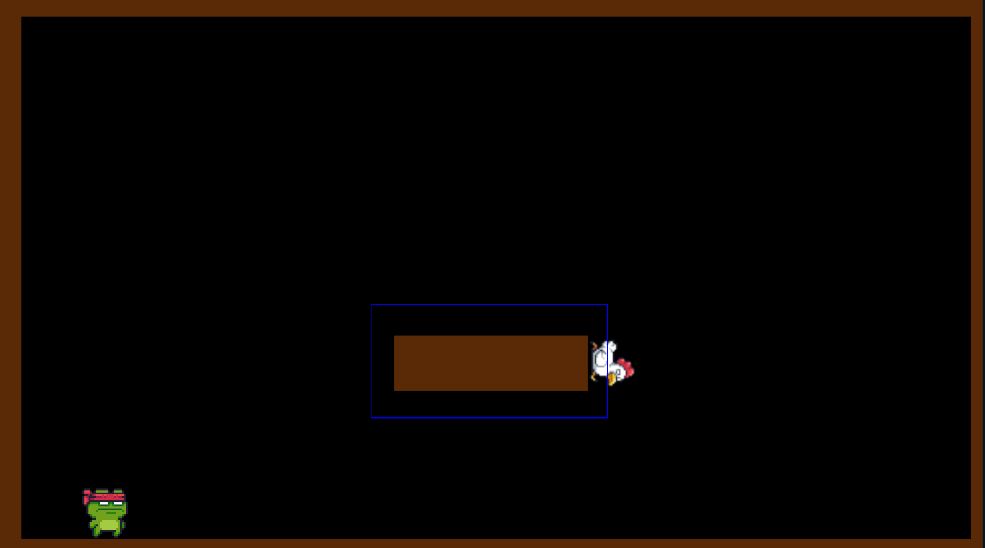
\includegraphics[height=5cm]{Imagenes/Gallina_Spline.png}
	\caption{Escena de ejemplo donde se aprecia una \textit{Spline Chicken} siguiendo su trayectoria.}
	\label{fig:SplineChicken}
\end{figure}

\subsection{Skywatch Eagle}

La \textit{Skywatch Eagle} (Figura~\ref{fig:SkywatchEagle}) es un ejemplo de enemigo con comportamiento reactivo, construido a partir de una máquina de estados. Su diseño combina movilidad aérea libre y un cambio abrupto hacia una acción ofensiva directa, lo que la convierte en una amenaza dinámica que exige atención constante por parte del jugador.\\

Este enemigo patrulla el cielo en un área determinada, recorriendo distintos puntos de forma aleatoria. Al detectar al jugador en su campo de visión, interrumpe su patrón y se lanza en picado hacia él. Este cambio de comportamiento genera un contraste entre una amenaza inicialmente pasiva y una reacción agresiva, lo que introduce tensión en el ritmo de juego.\\

Desde el punto de vista del diseño, la \textit{Skywatch Eagle} responde a dos intenciones clave: por un lado, introducir un enemigo volador que no se limita a un movimiento cíclico, sino que reacciona activamente a la presencia del jugador; y por otro, obligar al jugador a planificar su avance con más cuidado, ya que un movimiento en falso puede activar un ataque difícil de esquivar.\\

El comportamiento de este enemigo está compuesto por dos estados diferenciados:

\begin{itemize}
    \item \textbf{Estado 1 – Patrullaje aéreo:}  
    En este estado, el águila se desplaza de forma libre dentro de un área específica del escenario. La trayectoria entre puntos es fluida, y su movimiento tiene una función más disuasoria que ofensiva. Durante esta fase, observa el entorno en busca del jugador.

    \begin{itemize}
        \item \textit{Acción:} Movimiento entre posiciones aleatorias en el espacio aéreo.  
        \item \textit{Condición de transición:} Si el jugador se acerca lo suficiente, la enemiga cambia al estado de ataque.
    \end{itemize}

    \item \textbf{Estado 2 – Picado de ataque:}  
    Al entrar en este estado, la \textit{Skywatch Eagle} modifica radicalmente su comportamiento, lanzándose en picado hacia el jugador a gran velocidad. Durante este movimiento, su capacidad de infligir daño se activa. Tras el impacto, regresa al estado de patrullaje.

    \begin{itemize}
        \item \textit{Acción:} Desplazamiento rápido hacia la última posición detectada del jugador.  
        \item \textit{Condición de transición:} Al producirse el impacto con el jugador, retorna al estado de patrullaje.
    \end{itemize}
\end{itemize}

Este comportamiento se inspira directamente en patrones detectados en enemigos como la Vengamosca de \textit{Hollow Knight}, que combina movilidad aérea con un cambio de comportamiento agresivo al detectar al jugador. Esta dinámica se refleja también en la \textit{Skywatch Eagle}, cuya transición desde un patrullaje pasivo a un ataque en picado introduce una amenaza repentina y exige una respuesta rápida por parte del jugador. La inclusión de un estado de patrullaje previo refuerza el impacto del ataque y permite anticiparse, fomentando una experiencia de juego más estratégica.

\begin{figure}[t]
	\centering
	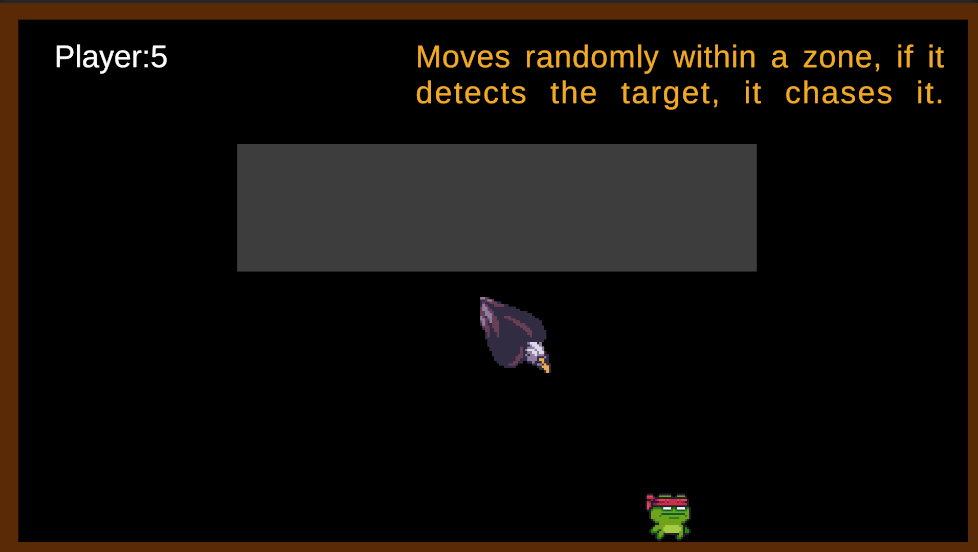
\includegraphics[height=5cm]{Imagenes/AguilaCayendo.png}
	\caption{Escena de ejemplo donde se aprecia a la \textit{Skywatch Eagle} atacando al jugador.}
	\label{fig:SkywatchEagle}
\end{figure}

\section{Conclusiones del Diseño}
En este capítulo, tras el análisis de enemigos en juegos de referencia como \textit{Hollow Knight}, \textit{Blasphemous} y \textit{Bzzzt}, se ha definido la arquitectura conceptual del framework para la creación de enemigos en 2D. Dicha definición se organiza en cuatro bloques fundamentales:

\begin{itemize}
  \item \textbf{Sensores}, responsables de detectar condiciones del entorno (presencia del jugador, colisiones, distancia, daño recibido).
  \item \textbf{Actuadores}, encargados de ejecutar acciones (movimientos lineales, circulares o spline, generación de unidades).
  \item \textbf{Módulo de daño}, que distingue entre emisión y recepción de daño, regulando cómo se inflige o recibe daño.
  \item \textbf{Máquina de Estados Finita}, que organiza los sensores y actuadores en estados coherentes y controla las transiciones entre ellos.
\end{itemize}

Asimismo, se ha incluido el mecanismo de sincronización con animaciones, que asocia cada estado de la FSM con la representación visual correspondiente, garantizando coherencia entre la lógica de IA y la experiencia del jugador.\\

Los ejemplos de diseño han validado la capacidad del framework para reproducir y combinar los patrones detectados en juegos comerciales, demostrando:

\begin{itemize}
  \item Modularidad en la composición de comportamientos.
  \item Escalabilidad en la complejidad de los enemigos.
  \item Claridad visual y diseño accesible para no programadores.
\end{itemize}

Con esta base conceptual completada, en el siguiente capítulo se desarrollará la implementación práctica de todos estos componentes en Unity para materializar el diseño teórico en una herramienta funcional.
